\vspace{10pt}
\section{Preliminaries and Motivations}

This section provides some preliminaries on ReRAM technology and cross-point architecture. Then the limitations of cross-point architecture are demonstrated by a series of simple example, which motivates the work in this paper.

\subsection{ReRAM technology and Cross-Point Architecture}

State of Art ReRAM technologies.

Memristor based ReRAM.

Cross-Point Architecture.

Sneak Path.
\begin{figure}
\centering
  % Requires \usepackage{graphicx}
  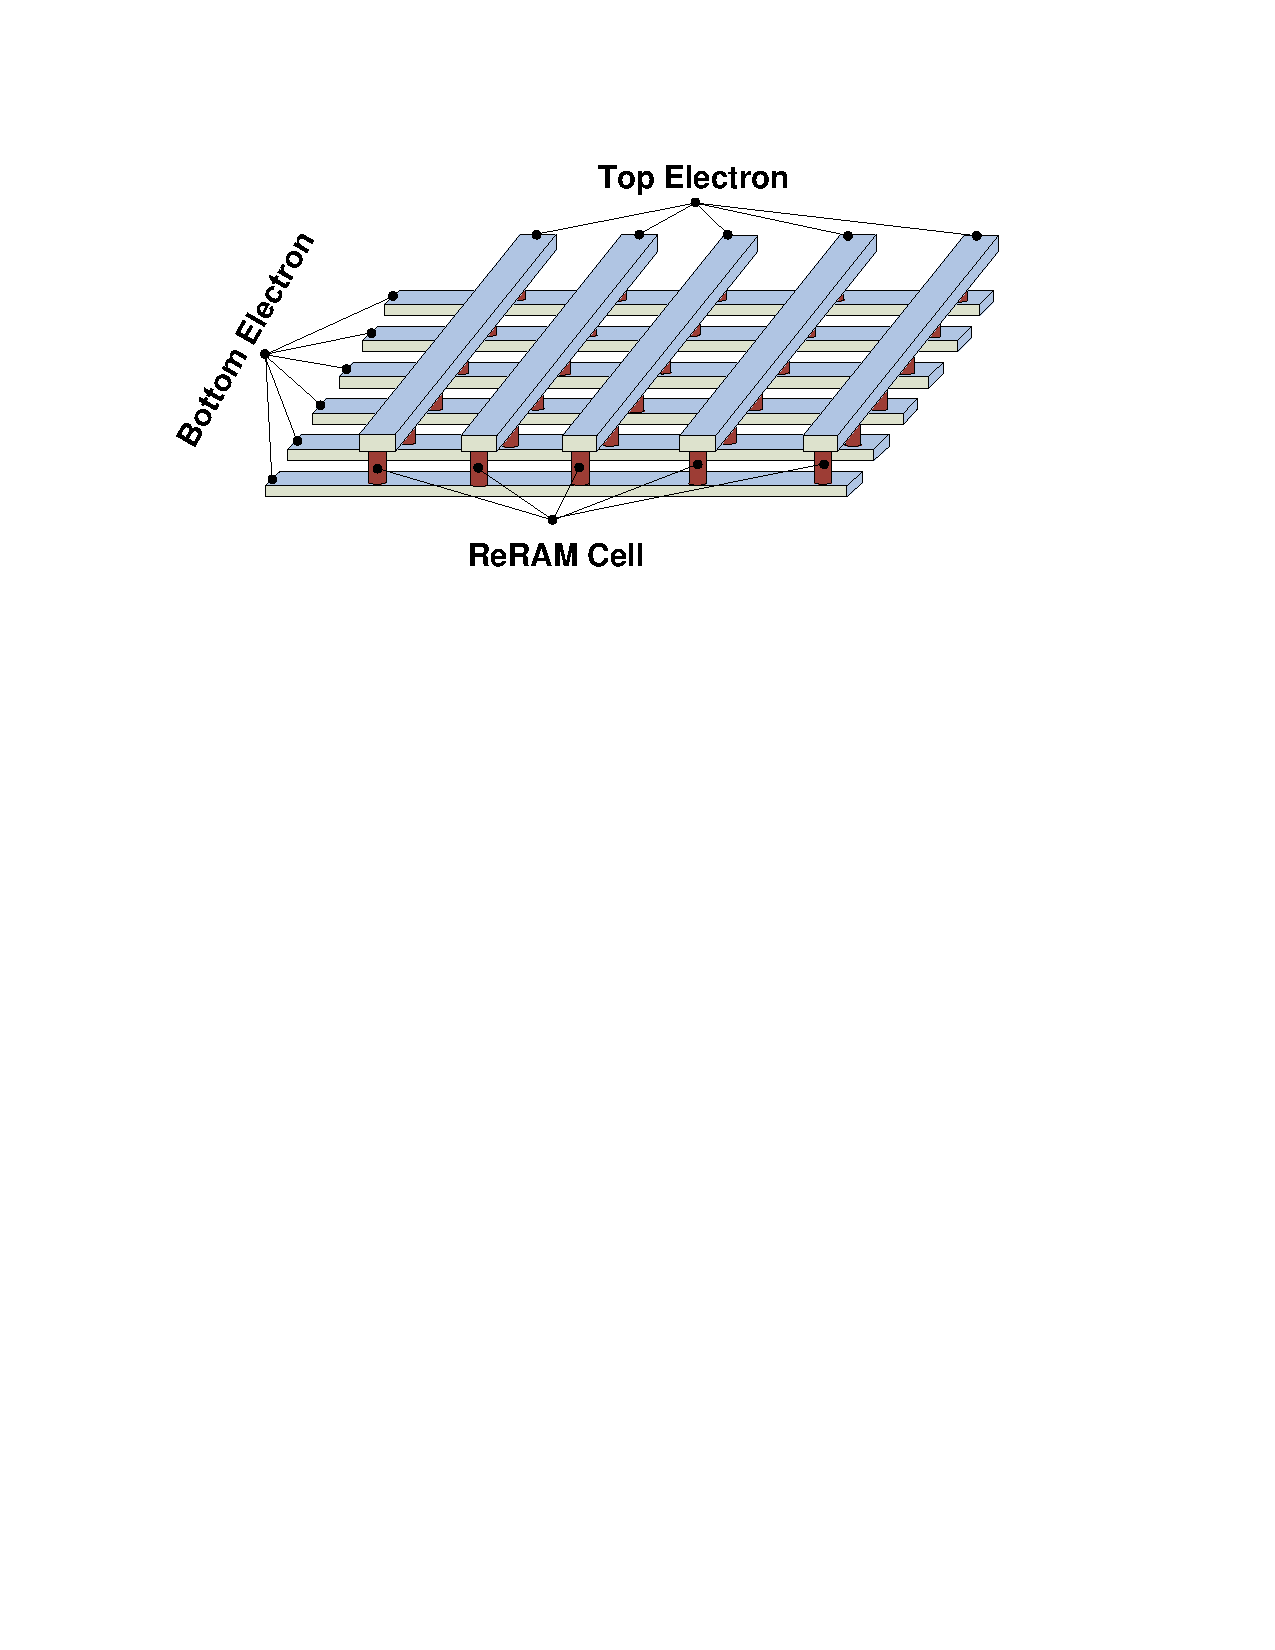
\includegraphics[width=0.45\textwidth]{./figures/crossbar_array.pdf}\\
  \caption{A schematic view of typical cross point architecture.}\label{fig:array}
\end{figure}

\subsection{Motivations}
As aforementioned, although the cross-point structure can provide the fabricate simplicity and area efficiency, it also incur lots of design challenges. Following cases show some examples to demonstrate the disadvantages of the cross-point structure, which motivates the work in this paper.
\begin{enumerate}
  \item \textbf{Reliable Write Operation}\\
  In order to 
  \item \textbf{Read Margin Disturb}\\
  123
  \item \textbf{Energy Waste Due to Sneak Pass}\\
  123
\end{enumerate}

~\cite{crossbar_NANO08_Nauenheim}~\cite{memristor:analog}~\cite{moore}

